%\documentclass{article}
\documentclass[openany,hebrew,ctexart]{book}
\usepackage{titletoc}
%\documentclass{cej}
\usepackage{fontspec}
\usepackage{xeCJK} %调用 xeCJK 宏包
%\setmainfont{BiauKai} %設定中文字型
%\setCJKmainfont{SimSun} %设置 CJK 主字体为 SimSun (宋体)
\setCJKmainfont{Noto Sans CJK TC}
\usepackage{fancyhdr}
%\usepackage{comment}
\usepackage{forest}
\usepackage{tabularx}
\usepackage[paper=portrait,pagesize]{typearea}
\usepackage{caption}
\usepackage{subcaption}
\usepackage{paracol}
\usepackage[utf8]{inputenc}
\usepackage{enumitem}
\usepackage{multirow}
\usepackage{etoolbox}
\usepackage{wrapfig,booktabs,threeparttable}
%\usepackage[subpreambles]{standalone}
\usepackage{pgfplots}
\usepackage{pgfplotstable}
%\pgfplotsset{
 %   width=matrix\textwidth,
%}
\usepackage{tikz}
\usetikzlibrary{snakes}
\usetikzlibrary{shapes.geometric,shapes.arrows,decorations.pathmorphing}
\usetikzlibrary{matrix,chains,scopes,positioning,arrows,fit,shapes.symbols}
\usetikzlibrary{calc,trees,positioning,decorations.pathreplacing,shapes}
\tikzset{
>=stealth',
  punktchain/.style={
    rectangle, 
    rounded corners, 
    % fill=black!10,
    draw=black, very thick,
    text width=10em, 
    minimum height=3em, 
    text centered, 
    on chain},
  line/.style={draw, thick, <-},
  element/.style={
    tape,
    top color=white,
    bottom color=blue!50!black!60!,
    minimum width=6em,
    draw=blue!40!black!90, very thick,
    text width=10em, 
    minimum height=3.5em, 
    text centered, 
    on chain},
  every join/.style={->, thick,shorten >=1pt},
  decoration={brace},
  tuborg/.style={decorate},
  tubnode/.style={midway, right=2pt},
}


\newenvironment{changemargin}[2]{%
\begin{list}{}{%
\setlength{\topsep}{-2pt}%
\setlength{\leftmargin}{20pt}%
\setlength{\rightmargin}{20pt}%
\setlength{\listparindent}{\parindent}%
\setlength{\itemindent}{\parindent}%
\setlength{\parsep}{\parskip}%
}%
\item[]}{\end{list}}


\usepackage{color}

\makeatother

\usepackage{mathtools}

\usepackage{tabularx}
\parindent=0pt
\defaultfontfeatures{Mapping=tex-text}
%\setmainfont[Ligatures=TeX]{Arial}
\usepackage[textwidth=16cm]{geometry}
\setlength{\parindent}{0pt}


\tikzstyle{decision} = [diamond, draw, fill=blue!20, 
    text width=4.5em, text badly centered, node distance=3cm, inner sep=0pt]
\tikzstyle{block} = [rectangle, draw, fill=blue!20, 
    text width=5em, text centered, rounded corners, minimum height=4em]
\tikzstyle{line} = [draw, -latex']
\tikzstyle{cloud} = [draw, ellipse,fill=red!20, node distance=3cm,
    minimum height=2em]


\usepackage{amssymb}
%\usepackage{array}
\newcolumntype{L}[1]{>{\raggedright\arraybackslash}p{#1}}









\DeclareCaptionLabelSeparator{emdash}{~--- }
\captionsetup[figure]{labelsep=emdash,font=onehalfspacing,position=bottom}
\captionsetup{%
    singlelinecheck=off,
    skip=2pt,
    justification=centering,
}

%我们可以通过 setspace宏包提供的命令来调整行间距。比如在导言区添加如下内容,可以将行距设置为字号的 1.5 倍:
\usepackage{setspace}
\onehalfspacing
 %在页眉左边写上我的名字,中间写上今天的日期,右边写上我的电话;页脚的正中写上页码;页眉和正文之间有一道宽为 0.4pt 的横线分割,可以在导言区加上如下几行
\usepackage{fancyhdr}
\pagestyle{fancy}
%\lhead{\author}
%\lhead{\thepage}
%\chead{\date}
\chead{\thepage}
\rhead{主日学}
\lfoot{}
%\cfoot{\thepage}
\rfoot{}
\renewcommand{\headrulewidth}{0.2pt}
\renewcommand{\headwidth}{\textwidth}
\renewcommand{\footrulewidth}{0pt}


%\title{你好,world!}
%\author{Liam}
%\date{}


%\renewcommand\thesection{\Roman{section}}
%\renewcommand\thesubsection{\Alph{subsection}}

\makeatletter
% #1 - comparator
% #2 - token list to sort
\newcommand\sort[2]{%
        \ifstrempty{#2}
        {}% else
        {%
                \sort@begin#1{}#2\sort@s\sort@begin
        }%
}

% helpers
\def\sort@s{\sort@s}
\def\ifsort@s#1{%
        \ifx\sort@s#1%
                \expandafter\@firstoftwo
        \else
                \expandafter\@secondoftwo
        \fi
}
% #1 - comparator
% #2 - tokens processed so far
% #3 - smallest token so far
% #4 - rest of the list
\def\sort@begin#1#2#3#4\sort@begin{%
        \ifsort@s{#4}
        {%
                \sortend{#3}%
                \sort#1{#2}%
        }% else
        {%
                \sort@go#1{#2}{#3}#4\sort@go
        }%
}

%     #1 - comparator
% #2 - tokens processed so far
% #3 - smallest token so far
% #4 - token under consideration
% #5 - rest of the list
\def\sort@go#1#2#3#4#5\sort@go{%
        #1{#3}{#4}{\sort@output#1{#2}{#5}}%
}
% #1 - comparator
% #2 - tokens processed so far
% #3 - rest of the list
% #4 - smaller of the two tokens
% #5 - larger of the two tokens
\def\sort@output#1#2#3#4#5{%
        \ifsort@s{#3}
        {%
                \sortoutput{#4}%
                \sort#1{#2{#5}}%
        }% else
        {%
                \sort@begin#1{#2{#5}}{#4}#3\sort@begin
        }%
}

\def\sort@numlt#1#2#3{%
        \ifnumcomp{#1}<{#2}
        {#3{#1}{#2}}% else
        {#3{#2}{#1}}%
}
\def\sort@numgt#1#2#3{%
        \ifnumcomp{#1}>{#2}
        {#3{#1}{#2}}% else
        {#3{#2}{#1}}%
}

\def\sort@alpha#1#2#3{%
        \ifnumcomp{\pdfstrcmp{#1}{#2}}<{0}
        {#3{#1}{#2}}% else
        {#3{#2}{#1}}%
}

\def\sort@firstcol#1#2{%
    \expandafter\expandafter\expandafter
        \sort@fc@helper\expandafter#1#2#1#2%
}

\def\sort@fc@helper#1&#2\\#3&#4\\#5#6#7{%
    \ifnumcomp{\pdfstrcmp{#1}{#3}}<{0}
    {#7{#5}{#6}}% else
    {#7{#6}{#5}}%
}

\newcommand*\sortnumlt{\sort\sort@numlt}
\newcommand*\sortnumgt{\sort\sort@numgt}
\newcommand*\sortalpha{\sort\sort@alpha}
\newcommand*\sortfirstcol{\sort\sort@firstcol}
\makeatother

% Change these to change out the sort outputs.
\newcommand*\sortoutput[1]{#1}
\newcommand*\sortend[1]{#1}







\KOMAoptions{paper=portrait,pagesize}
\recalctypearea
%设置页边距,推荐使用 geometry 宏包。可以在这里查看它的说明文档
\usepackage{geometry}
\geometry{papersize={17cm,15cm}}
\geometry{left=1.5cm,right=2.cm,top=1.cm,bottom=1cm}
%\usepackage[margin=0.5in]{geometry}
\addtolength{\oddsidemargin}{-.15075in}
\addtolength{\evensidemargin}{-.15075in}
\addtolength{\textwidth}{0.75in}

\addtolength{\topmargin}{0.275in}
\addtolength{\textheight}{1.75in}
\geometry{
 a4paper,
 total={190mm,257mm},
 left=15mm,
 top=20mm,
 }
 
 %4 level 
\usepackage{titlesec}
\setcounter{secnumdepth}{4}
\titleformat{\paragraph}
{\normalfont\normalsize\bfseries}{\theparagraph}{1em}{}
\titlespacing*{\paragraph}
{0pt}{3.25ex plus 1ex minus .2ex}{1.5ex plus .2ex}
 
\rfoot{Page \thepage \hspace{1pt} of \pageref{LastPage}} 

\titlespacing{\section}{0.2pt}{\parskip}{-\parskip}
\titlespacing{\subsection}{0.2pt}{\parskip}{-\parskip}
\titlespacing{\subsubsection}{0.2pt}{\parskip}{-\parskip}

%\titlespacing\section{0pt}{12pt plus 2pt minus 8pt}{0pt plus 2pt minus 8pt}
\titlespacing\subsection{0pt}{12pt plus 2pt minus 8pt}{0pt plus 2pt minus 8pt}
\titlespacing\subsubsection{0pt}{12pt plus 2pt minus 8pt}{0pt plus 2pt minus 8pt}

\usepackage[toc,page]{appendix}
\usepackage{caption}
\usepackage{subcaption}
%\usepackage{subfig}
\usepackage{graphicx}
\usepackage{smartdiagram}
\usepackage{cjhebrew} 
\usepackage{float}%table{H}


\titleclass{\subsubsubsection}{straight}[\subsection]
\newcounter{subsubsubsection}[subsubsection]
\renewcommand\thesubsubsubsection{\thesubsubsection.\arabic{subsubsubsection}}
\renewcommand\theparagraph{\thesubsubsubsection.\arabic{paragraph}} % optional; useful if paragraphs are to be numbered
\titleformat{\subsubsubsection}
  {\normalfont\normalsize\bfseries}{\thesubsubsubsection}{1em}{}
\titlespacing*{\subsubsubsection}
{0pt}{3.25ex plus 1ex minus .2ex}{1.5ex plus .2ex}
\makeatletter
\renewcommand\paragraph{\@startsection{paragraph}{5}{\z@}%
  {3.25ex \@plus1ex \@minus.2ex}%
  {-1em}%
{\normalfont\normalsize\bfseries}}
\renewcommand\subparagraph{\@startsection{subparagraph}{6}{\parindent}%
  {3.25ex \@plus1ex \@minus .2ex}%
  {-1em}%
  {\normalfont\normalsize\bfseries}}
\def\toclevel@subsubsubsection{4}
\def\toclevel@paragraph{5}
\def\toclevel@paragraph{6}
\def\l@subsubsubsection{\@dottedtocline{4}{7em}{4em}}
\def\l@paragraph{\@dottedtocline{5}{10em}{5em}}
\def\l@subparagraph{\@dottedtocline{6}{14em}{6em}}
\makeatother

\setcounter{secnumdepth}{4}
\setcounter{tocdepth}{3}
\usepackage{verbatim}%\begin{document}\end{comment}
\usepackage{colortbl}

\usepackage{rotating}%sidewaystable}

\usepackage{hyperref}
\hypersetup{
    colorlinks=true,
    linkcolor=blue,
    filecolor=magenta,      
    urlcolor=cyan,
    pdftitle={Sharelatex Example},
    bookmarks=true,
    pdfpagemode=FullScreen,
}
\urlstyle{same}
\colorlet{TEAL}{red}
\begin{document}


%============================================
%    目錄,圖目錄,表目錄
%============================================
\renewcommand\contentsname{目錄}
\renewcommand\listfigurename{圖目錄}
\renewcommand\listtablename{表目錄}
\tableofcontents
\thispagestyle{empty}
\listoffigures
\thispagestyle{empty}
\listoftables
\thispagestyle{empty}

\makeatletter
\let\origsection\section
\renewcommand\section{\@ifstar{\starsection}{\nostarsection}}
\newcommand\nostarsection[1]
{\sectionprelude\origsection{#1}\sectionpostlude}
\newcommand\starsection[1]
{\sectionprelude\origsection*{#1}\sectionpostlude}
\newcommand\sectionprelude{%
  \vspace{.5em}
}
\newcommand\sectionpostlude{%
  \vspace{0em}
}
\makeatother






%\tableofcontents

\section{问题}
\subsection{挪亚洪水启示我们:神在审判之前先通知义人(挪亚)审判的消息。为什么主耶稣来到的日子要像夜间的贼?}
“主的日子来到好像夜间的贼"出自帖前5:1-8,“你们自己明明晓得,主的日子来到好像夜间的贼一样。人正说平安稳妥的时候,灾祸忽然临到\textcolor{blue}{他们},如同产难临到怀胎的妇人一样,\textcolor{blue}{他们}绝不能逃脱
。\textcolor{red}{弟兄们,你们},\textcolor{red}{你们}却不在黑暗里,叫那日子临到\textcolor{red}{你们}像贼一样。\textcolor{red}{你们}都是光明之子,都是白昼之子。\textcolor{red}{我们}不是属黑夜的,也不是属幽暗的。所以,\textcolor{red}{我们}不要睡觉,像别人一样,总要警醒谨守。 因为睡了的人是在夜间睡,醉了的人是在夜间醉。 但\textcolor{red}{我们}既然属乎白昼,就应当谨守,把信和爱当做护心镜遮胸,把得救的盼望当做头盔戴上"。
\setlist{nolistsep}
\begin{itemize}[noitemsep]
\item 对于“他们(不认识主的人)",主的日子来到确实好像夜间的贼一样
\begin{itemize}[noitemsep]
\item 主是忽然临到,因为主是在众人都说“平安稳妥的时候”来到。
\item 就如同睡觉的人在黑暗中看不清盗贼的脸一样,主耶稣的到来,“他们"也完全不知道。
\end{itemize}
\item 对于“你们/我们(光明之子)",只要我们警醒谨守,主的日子来到是在光明中
\end{itemize}

\subsection{我们将来所得的国度是虚拟(灵里)的,还是真实的在地上的?}
\begin{itemize}[noitemsep]
\item 我们现在得到的是属灵的福气:天上的耶路撒冷。
\begin{itemize}[noitemsep]
\item 加4:22-26 律法上記著,亞伯拉罕有兩個兒子,一個是使女生的,一個是自主之婦人生的。然而那使女所生的是按著血氣生的,那自主之婦人所生的是憑著應許生的。這都是比方:那兩個婦人就是兩約。一約是出於西奈山,生子為奴,乃是夏甲。這夏甲二字是指著阿拉伯的西奈山,與現在的耶路撒冷同類,因耶路撒冷和她的兒女都是為奴的。但那\underline{在上的耶路撒冷是自主的,她是我們的母}。
\item 彼前1:3 父神曾照自己的大憐憫,藉著耶穌基督從死裡復活重生了我們,叫我們有活潑的盼望,可以得著不能朽壞、不能玷汙、不能衰殘、為你們存留在\underline{天上的基業}。
\item 彼前2:4-5 主乃活石,固然是被人所棄的,卻是被神所揀選、所寶貴的。你們來到主面前,也就像\underline{活石},被建造\underline{成為靈宮},做聖潔的祭司,藉著耶穌基督奉獻神所悅納的靈祭。
\end{itemize}
\item 到主耶稣再来的时候,我们将承受神给亚伯拉罕的应许。\\
“你們因信基督耶穌,都是神的兒子。你們受洗歸入基督的,都是披戴基督了;並不分猶太人、希臘人,自主的、為奴的,或男或女,因為你們在基督耶穌裡都成為一了。你們\underline{既屬乎基督,就是亞伯拉罕的後裔,是照}\\
\underline{著應許承受產業的了(加4:26-29)}"。
\item 圣经中有许多关于千年国度的描述,列举部分供参考
\begin{itemize}[noitemsep]
\item 可能因为末后有许多地震,导致耶路撒冷成为世界上最高的山.\\
“末后的日子,耶和华殿的山必坚立超乎诸山,高举过于万岭,万民都要流归这山(賽2:2/彌4:1-3)。"
\item 以西结书40-48章提到,千年国度会重建圣殿,参考Figure 1(\ref{fig:sub1}\footnotetext{https://cmcbiblereading.com/wp-content/uploads/2021/09/Temple-Sizes-Comparison-1024x717.png})是以西结异象中的圣殿与摩西会幕、所罗门圣殿和希律圣殿的尺寸比较;并重新分配土地,参考Figure 2(\ref{fig:sub2}\footnotetext{https://cmcbiblereading.com/wp-content/uploads/2021/09/The-Sanctuary-Portion-1024x797.png})以色列「当献的供地」示意图。
\item 在那个时候,除了基督的国度,世界上还有其他的国家.这些战后得以进入千年国度的人们,每年7月15-22号都要来耶路撒冷过住棚节。\\
“所有來攻擊耶路撒冷列國中剩下的人,必年年上來敬拜大君王萬軍之耶和華,並守住棚節。地上萬族中,凡不上耶路撒冷敬拜大君王萬軍之耶和華的,必無雨降在他們的地上。埃及族若不上來,雨也不降在他們的地上。凡不上來守住棚節的列國人,耶和華也必用這災攻擊他們。這就是埃及的刑罰和那不上來守住棚節之列國的刑罰。當那日,馬的鈴鐺上必有「歸耶和華為聖的」這句話。耶和華殿內的鍋必如祭壇前的碗一樣。凡耶路撒冷和猶大的鍋都必歸萬軍之耶和華為聖,凡獻祭的都必來取這鍋,煮肉在其中。當那日,在萬軍之耶和華的殿中必不再有迦南人(撒迦利亞書14:16-20)。"
\end{itemize} 
\end{itemize}
%https://cmcbiblereading.com/wp-content/uploads/2021/09/The-Sanctuary-Portion-1024x797.png

\begin{figure} 
\centering
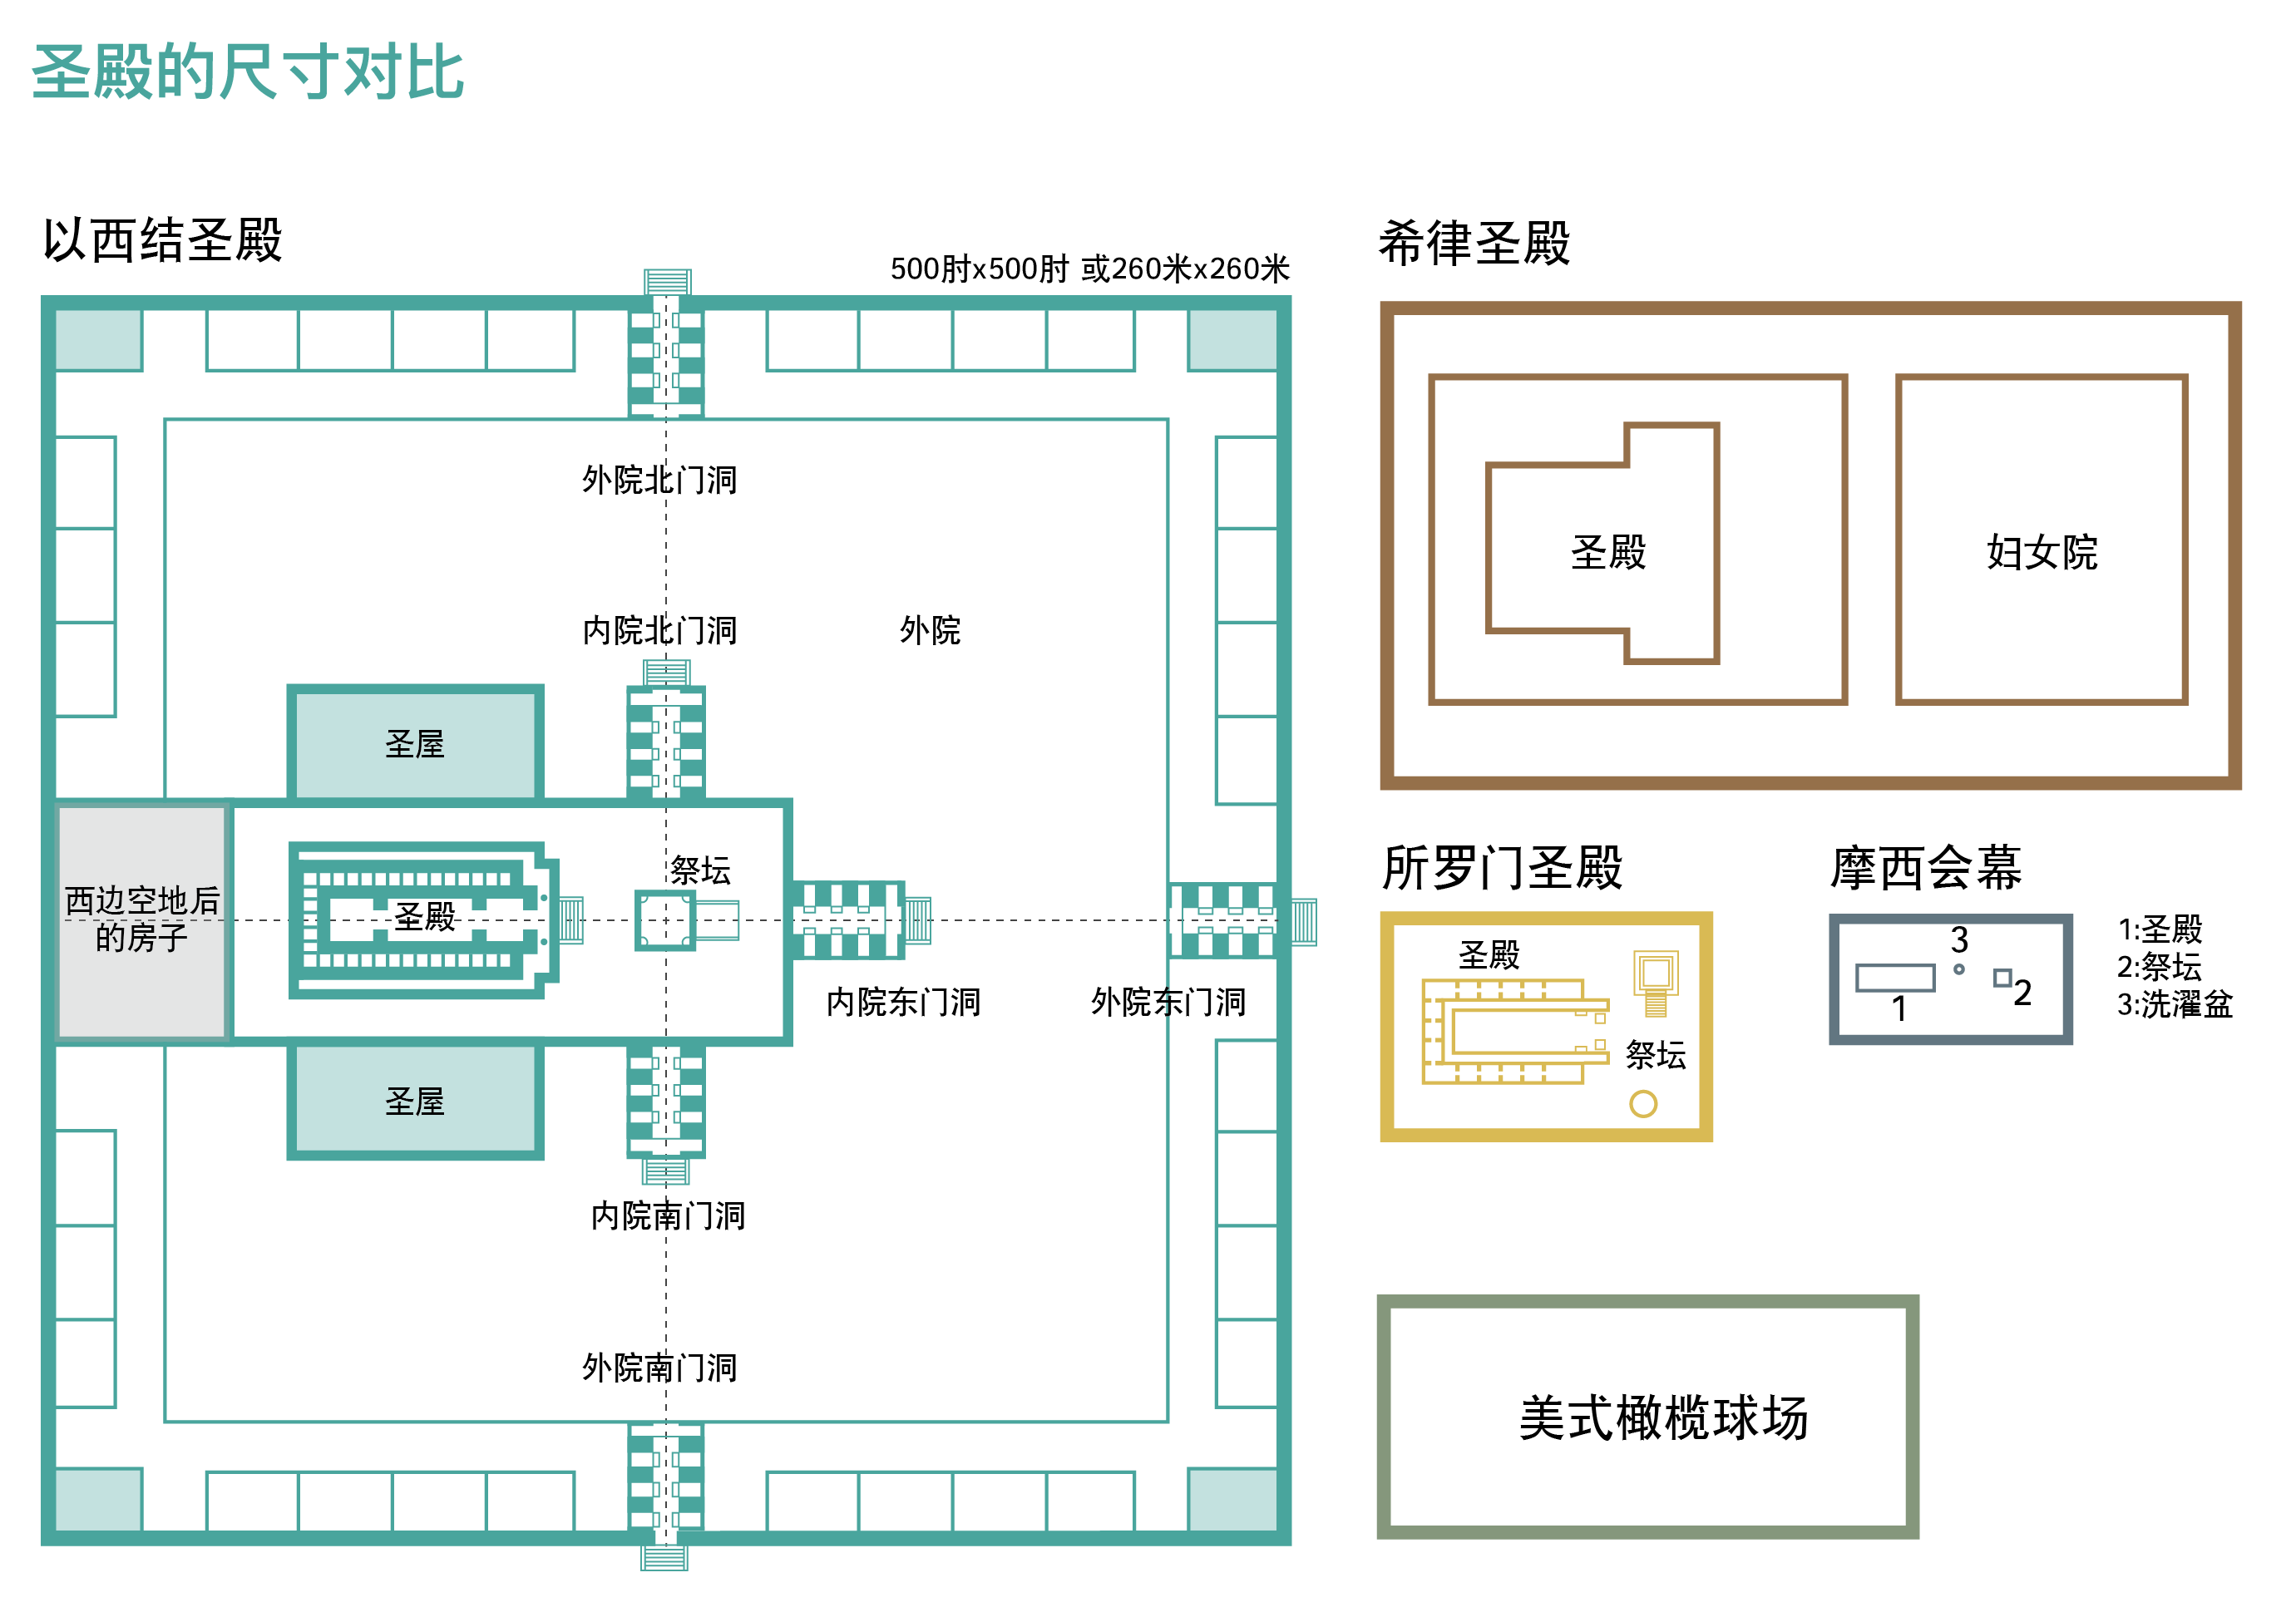
\includegraphics[width=5in]{TempleSizesComparison.png}
\caption{以西结异象中的圣殿与摩西会幕、所罗门圣殿和希律圣殿的尺寸比较}
\label{fig:sub1}
\end{figure} 

\begin{figure} 
\centering
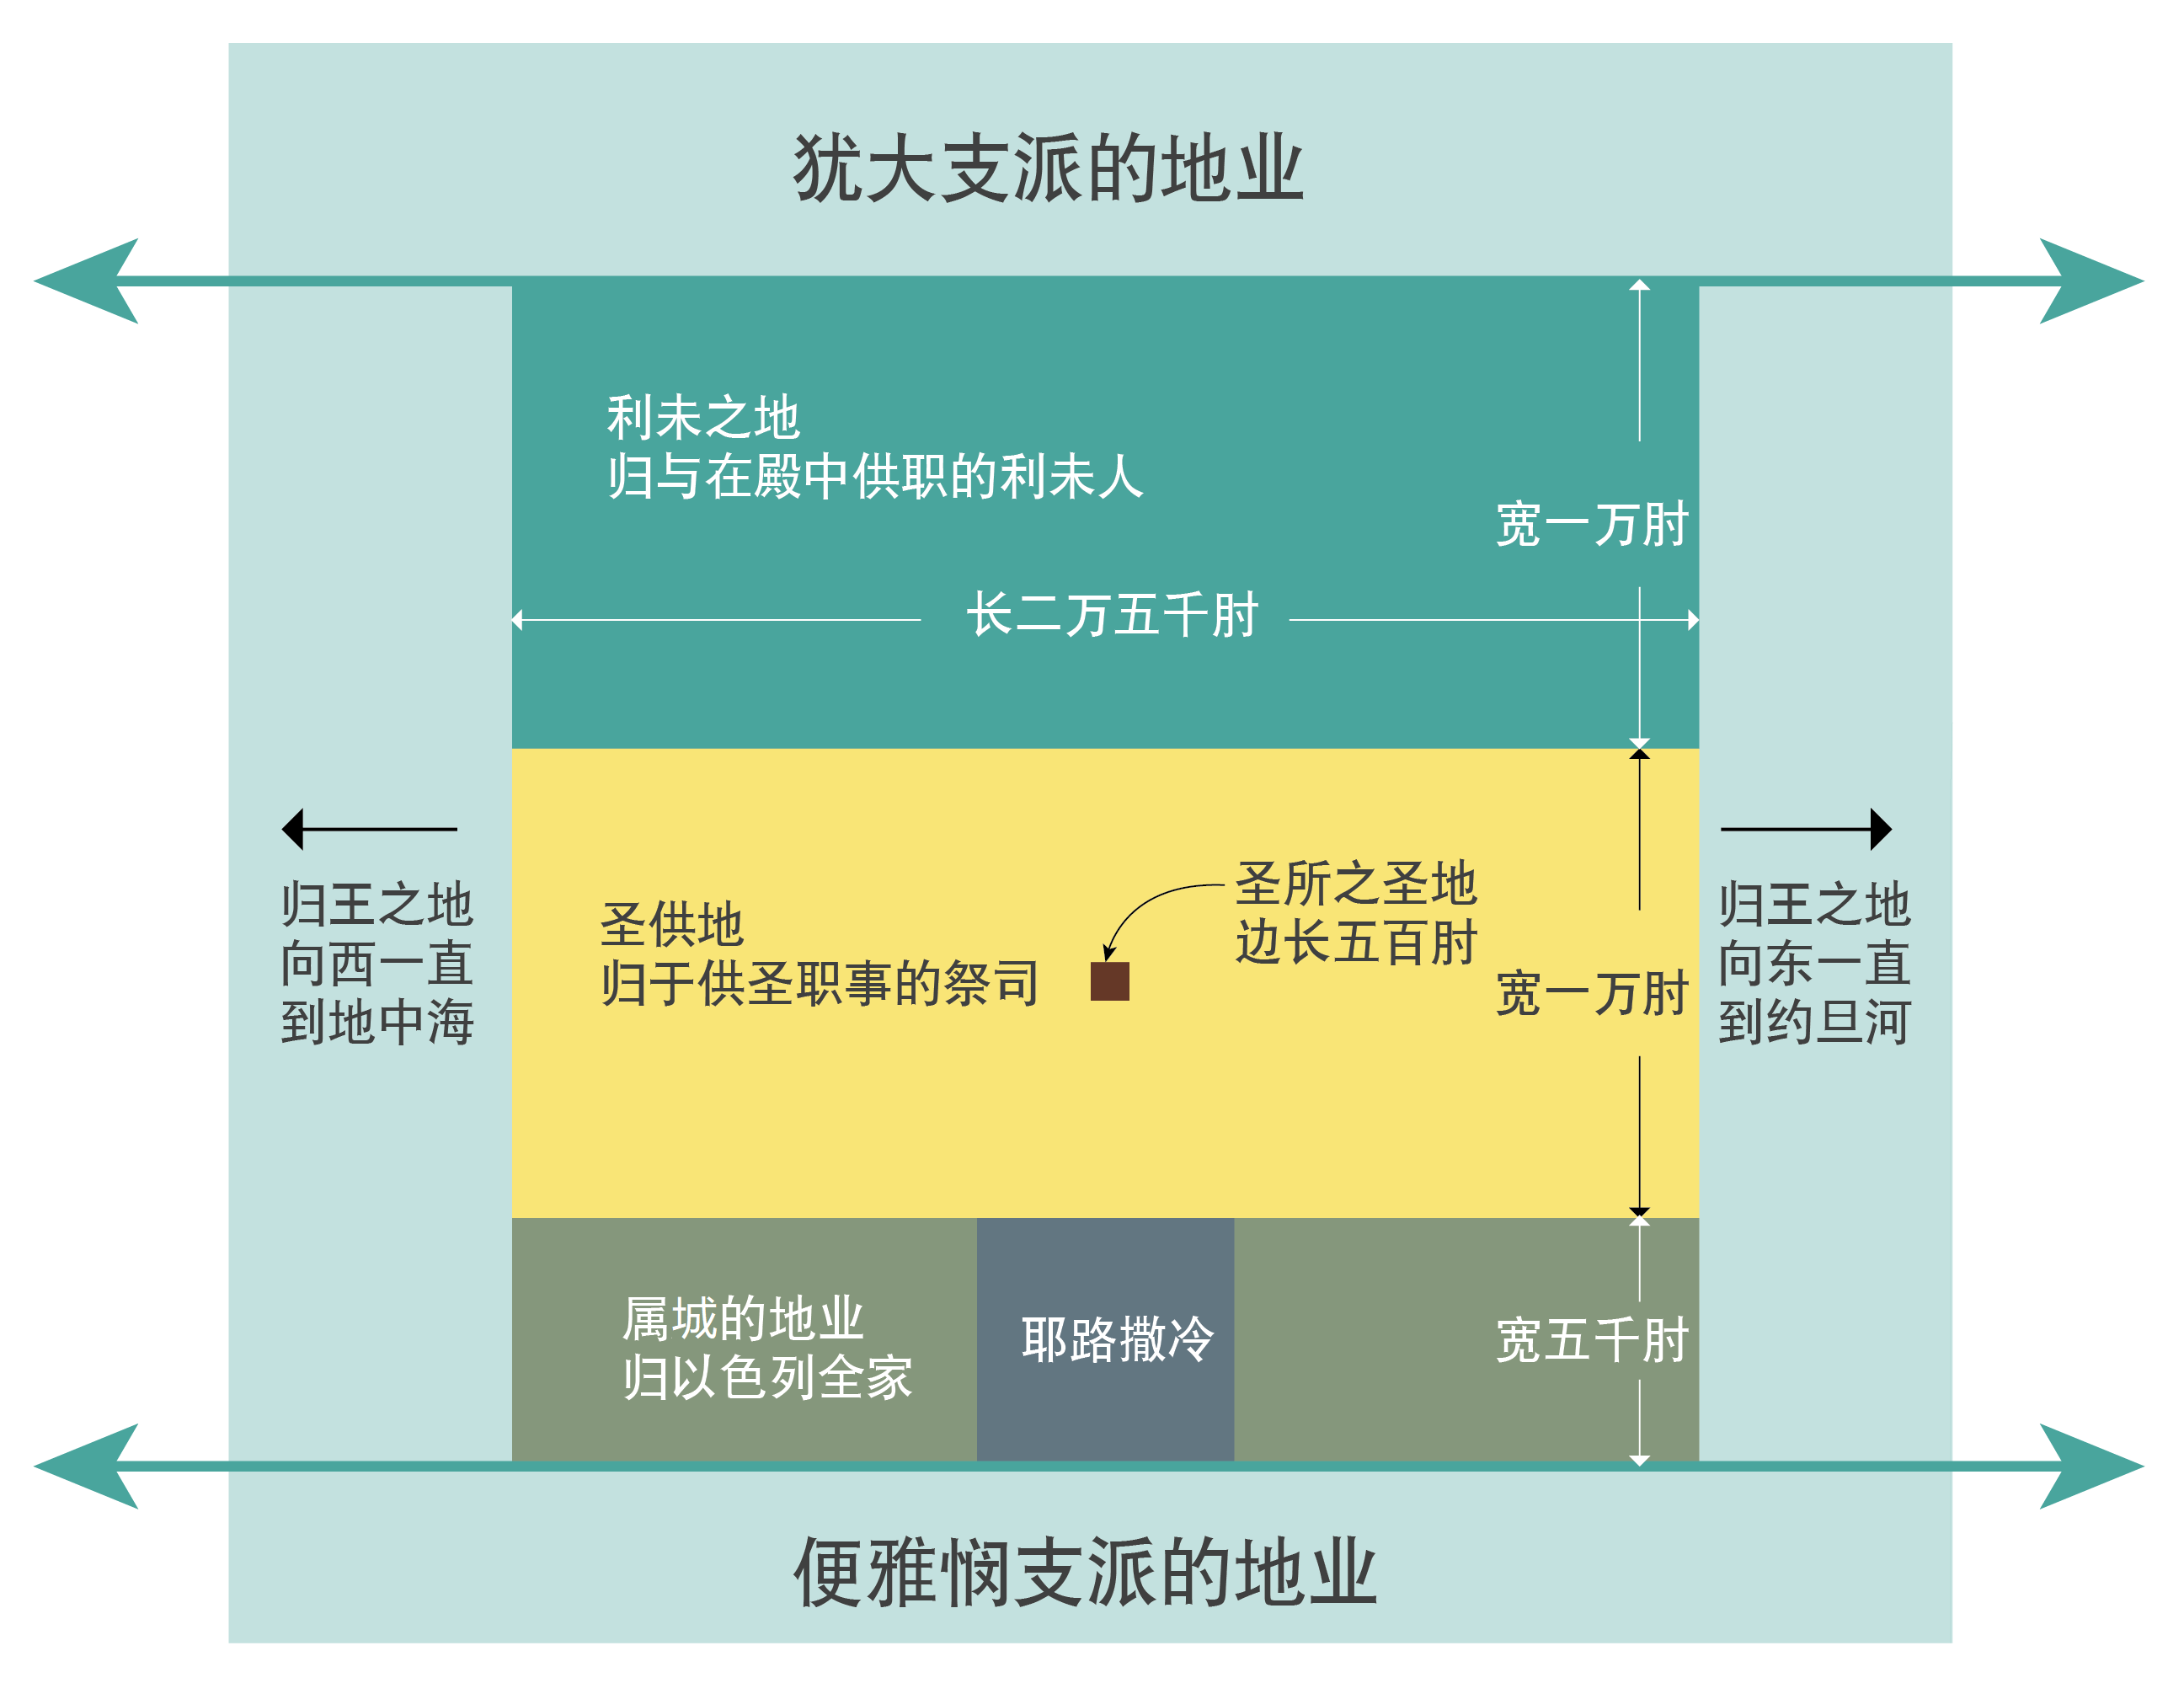
\includegraphics[width=5in]{land.png}
\caption{以西结异象里以色列「当献的供地」}
\label{fig:sub2}
\end{figure} 


\end{document}
